\documentclass[11pt]{article}
\usepackage{../header}

\def\title{Transistors}

\begin{document}
\maketitle
\tableofcontents
\newpage

\section{Switches}

Switches in circuitry denote a boolean value: either "off" (0) or "on" (1). More specifically, there are three components to a switch: the source ($S$), drain ($D$), and gate ($G$).

When the gate is in its "on" state, the switch is closed, and current passes between the source and the drain. Otherwise, no current flows. 

\begin{figure}[H]
    \centering
        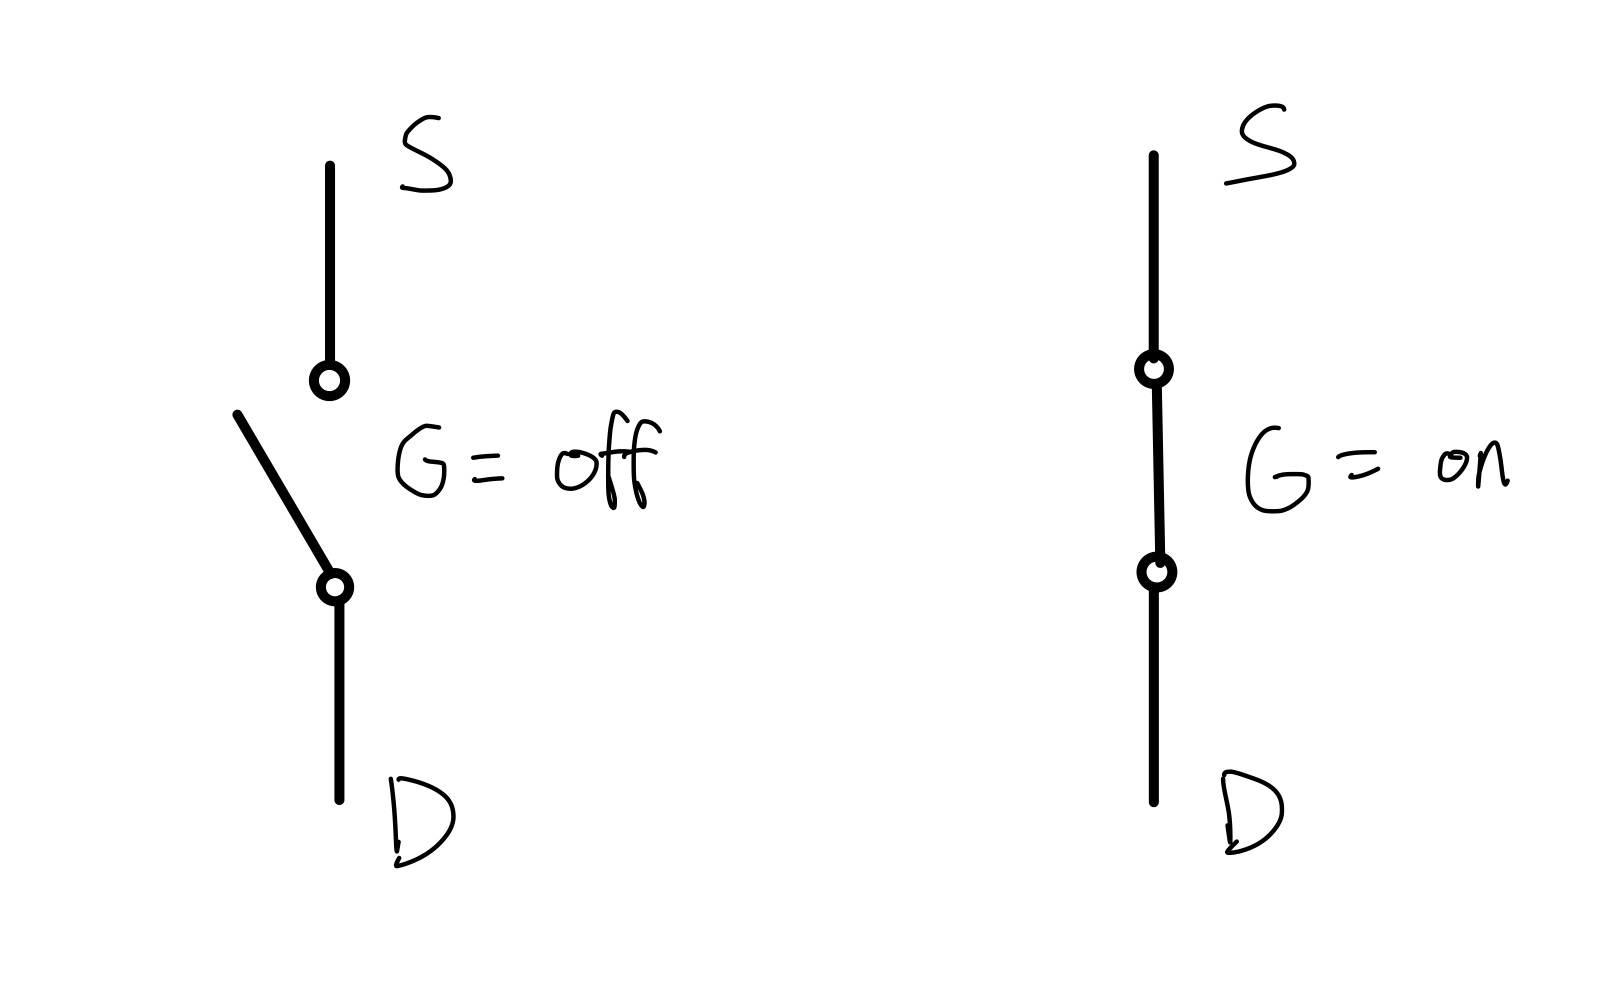
\includegraphics[scale=.1]{01-transistors/switch.jpeg}
    \caption{Switch circuit model}
\end{figure}

\section{PMOS and NMOS transistors}

In the most simplified form, transistors are switches whose gate is controlled by a threshold gate voltage, measured as the voltage at the gate ($V_G$) relative to the voltage at the source ($V_S$). We denote this voltage as $V_{GS}=V_G-V_S$ and its negation $V_{SG}=-V_{GS}=V_S-V_G$.

In this class, we will cover the CMOS family of transistors, which consist of two types: PMOS and NMOS. Each has a different condition for closing its switch:
\begin{itemize}
    \item NMOS: when the gate voltage is greater than some positive threshold $V_{tn}$. In other words, $V_{GS}>V_{tn}$
    \item PMOS: when the gate voltage is less than some negative threshold $-V_{tp}$. In other words, $V_{GS}<-V_{tp}$ or $V_{SG}>V_{tp}$
\end{itemize}

\begin{figure}[H]
    \centering
        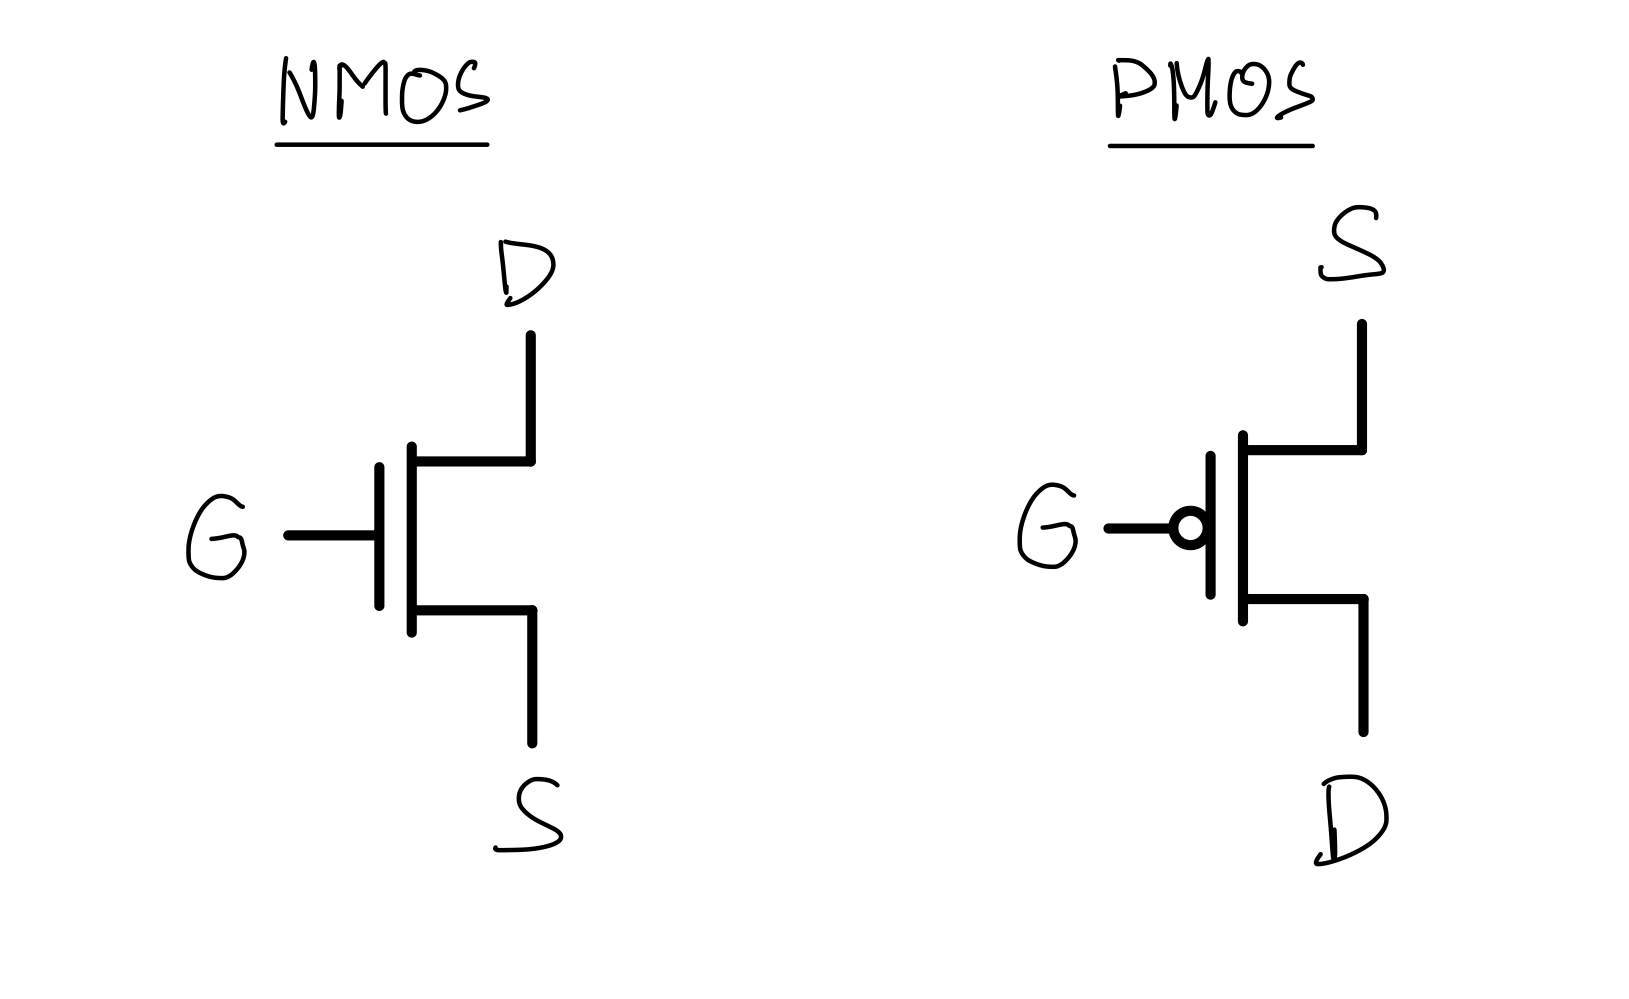
\includegraphics[scale=.12]{01-transistors/transistor-circuits.jpeg}
    \caption{CMOS transistors circuit model}
\end{figure}

\subsection{Transistor physics}

However, transistors are not actually that simple. While an exact model of involves an extensive knowledge in physics and is out of scope for this class, a "charge puddle" model of the transistor can provide us with more detail on how they work.

\begin{figure}[H]
    \centering
        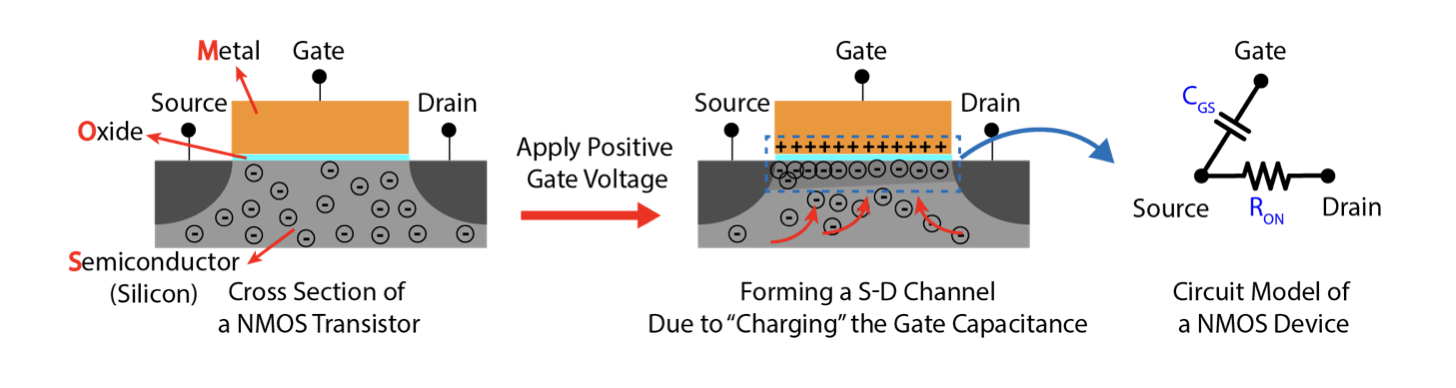
\includegraphics[scale=.5]{01-transistors/nmos-diagram.png}
    \caption{Puddle model of a transistor}
\end{figure}

The gate and the silicon connecting the source and drain act similar to two ends of a capacitor. An increase in voltage on the gate causes a "puddle" of charge carriers to form on the silicon, which increases until it is large enough to connect the source and drain, allowing current to pass between them. The gate voltage that corresponds to that connection is the threshold voltage. 

\subsection{Resistor-switch model}

With the charge puddle model in mind, we can construct a better circuit model of the transistor. Since the puddle is not a perfect conductor, there is some resistance between the source and drain of a transistor when they are connected. Additionally, we noted earlier that the gate and silicon acted similar to a capacitor, so we add a capacitor between the gate and the source. 

\begin{figure}[H]
    \centering
        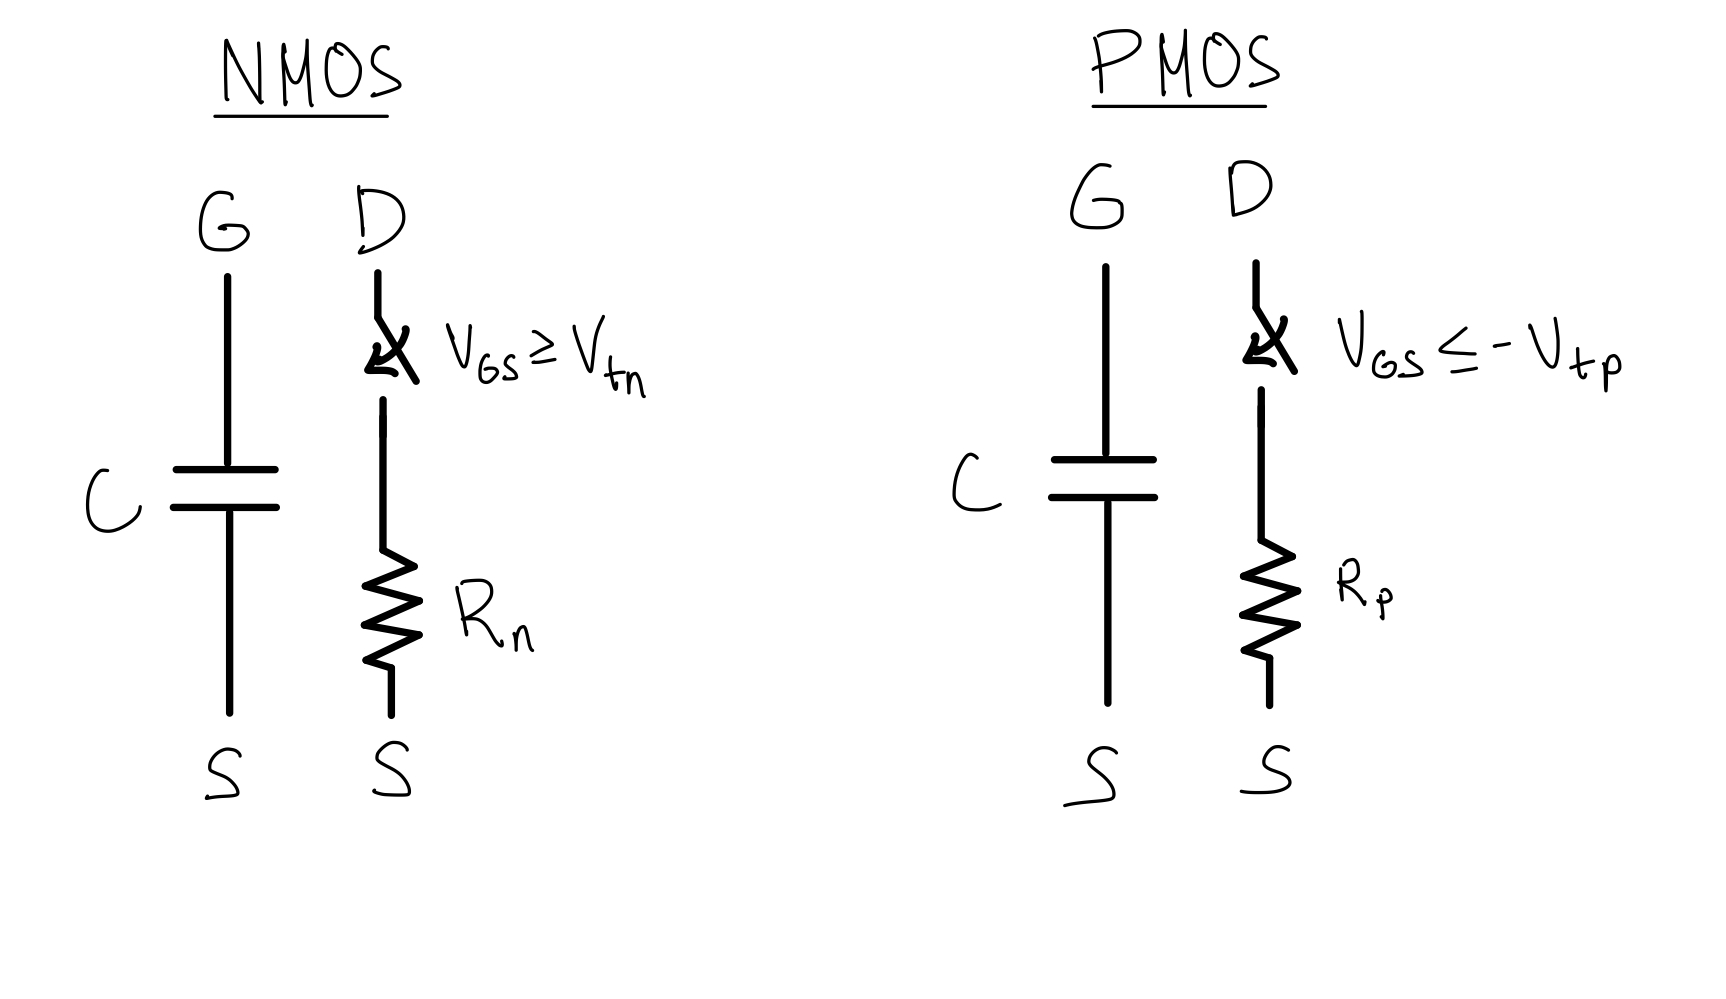
\includegraphics[scale=.15]{01-transistors/resistor-switch.jpeg}
    \caption{Resistor-switch model of CMOS transistors}
\end{figure}

As we will see soon, we can use this model to observe some interesting behaviors in circuits involving transistors.

\newpage
\section{Inverters}

An inverter is a circuit component that does a "NOT" operation: it maps a 0 (low) input to a 1 (high) output and vice versa. Physically, it's composed of an NMOS and a PMOS transistor that are connected together as such:

\begin{figure}[H]
    \centering
        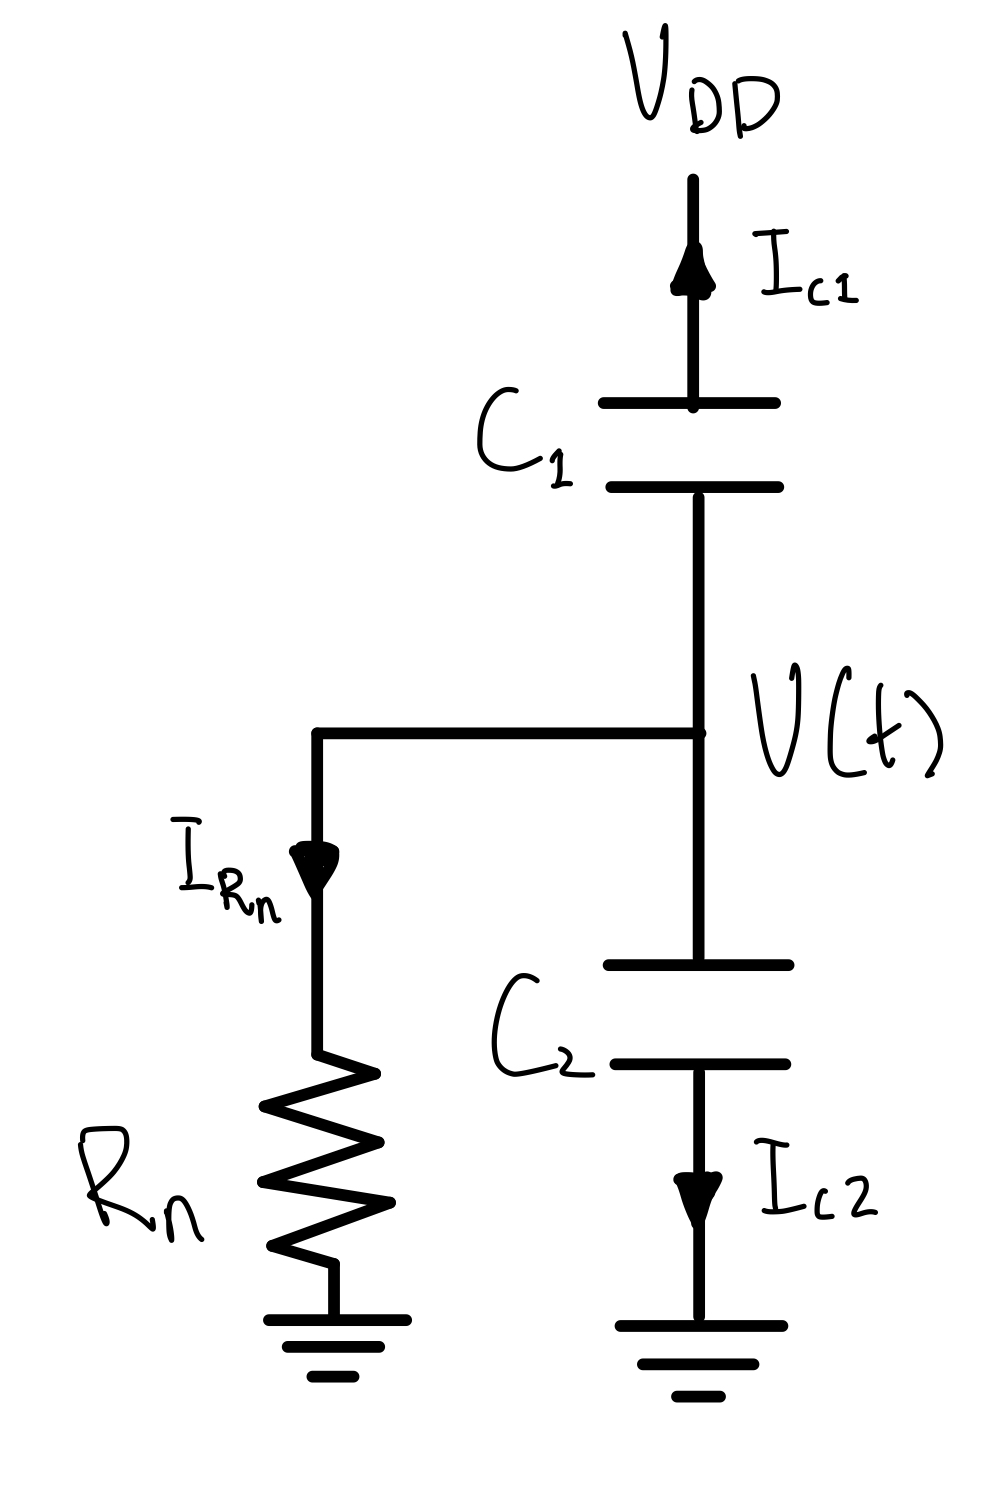
\includegraphics[scale=.12]{01-transistors/inverter.jpeg}
    \caption{CMOS inverter}
\end{figure}

For the PMOS transistor, the gate voltage is $V_{SG_p}=V_{DD}-V_{in}$. For our NMOS transistor, it is $V_{GS_n}=V_{in}-0$. 

When the input voltage is high (specifically when $V_{in}>V_{tn}$), the NMOS transistor closes its switch, so ground and $V_{out}$ are connected.

On the other hand, when the input voltage is low (specifically when $V_{in}<V_{DD}-V_{tp}$, and thus $V_{SG_p}>V_{tp}$), the PMOS transistor closes its switch, so $V_{DD}$ and $V_{out}$ are connected.

\section{Oscillators}

Now, what if we chain an odd number of inverters together into a loop? If we do that, we create what is called an oscillator. 

\begin{figure}[H]
    \centering
        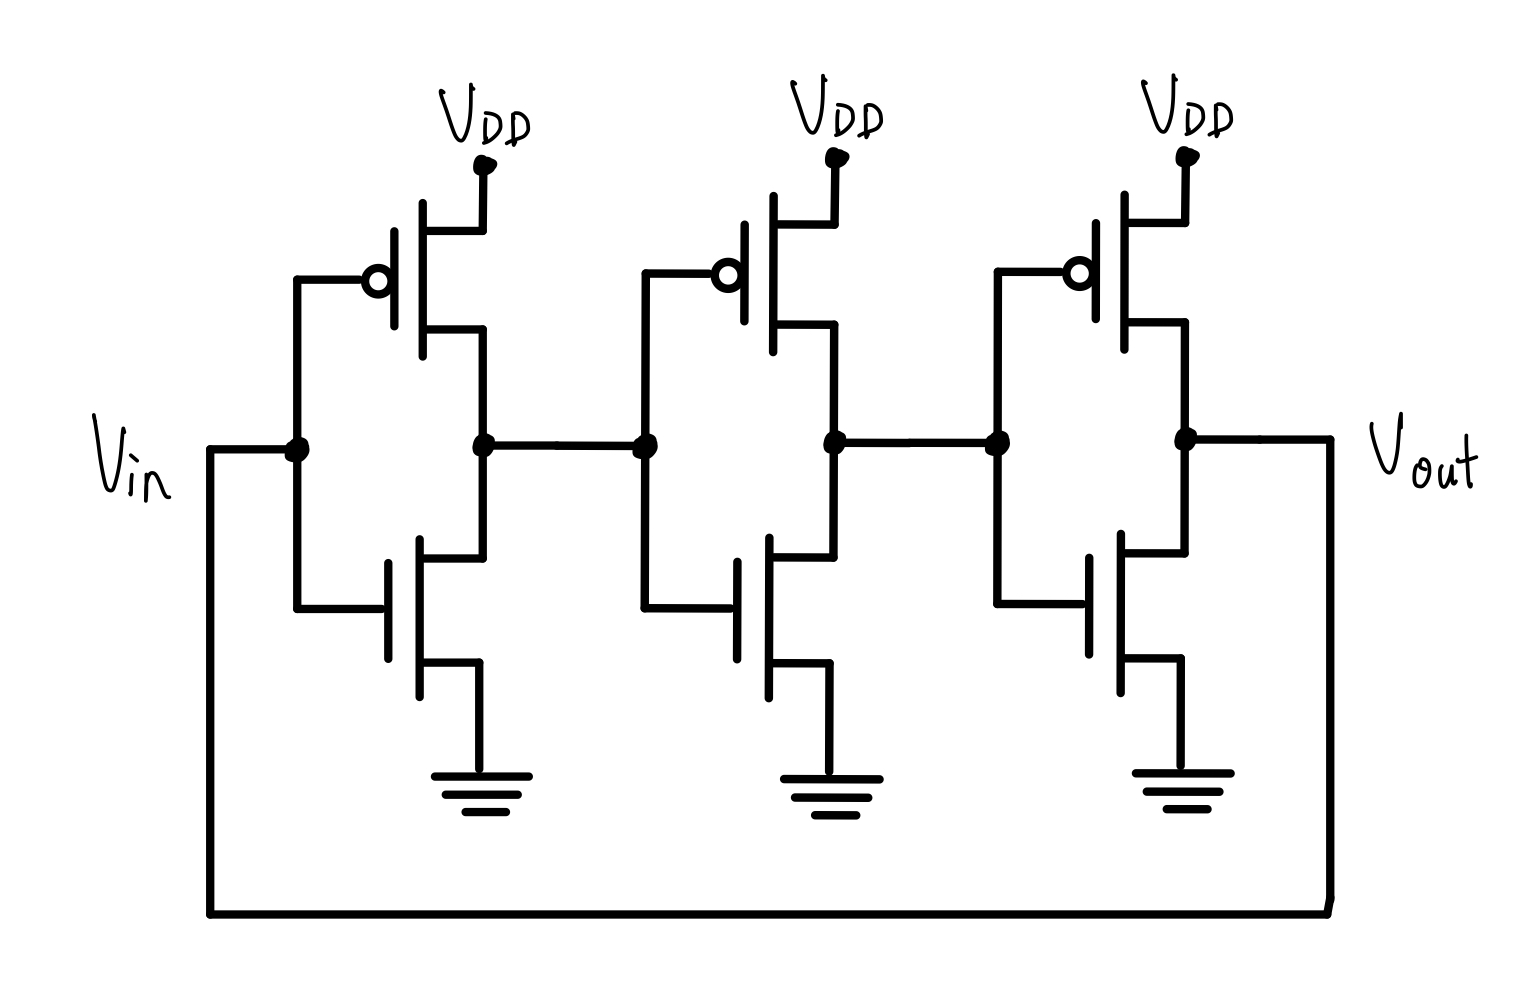
\includegraphics[scale=.14]{01-transistors/oscillator.jpeg}
    \caption{Ring oscillator with 3 CMOS inverters}
\end{figure}

As the name implies, the voltage of this system oscillates between high and low, and it does so at some constant frequency. That makes it useful for clocks and other digital devices.

We won't prove this here, but you need more than one inverter, otherwise it could converge to some intermediate value. For best results, an odd prime number of inverters should be used due to properties with modular arithemtic. 

\subsection{Detailed model}
The reason why an oscillator actually oscillates is because the inverters do not immediately invert their voltages, creating a chain of sequential inversions that happen on a delay. 

Let's revisit the resistor-switch model of the transistor to take a closer look at why this is the case. 

\begin{figure}[H]
    \centering
        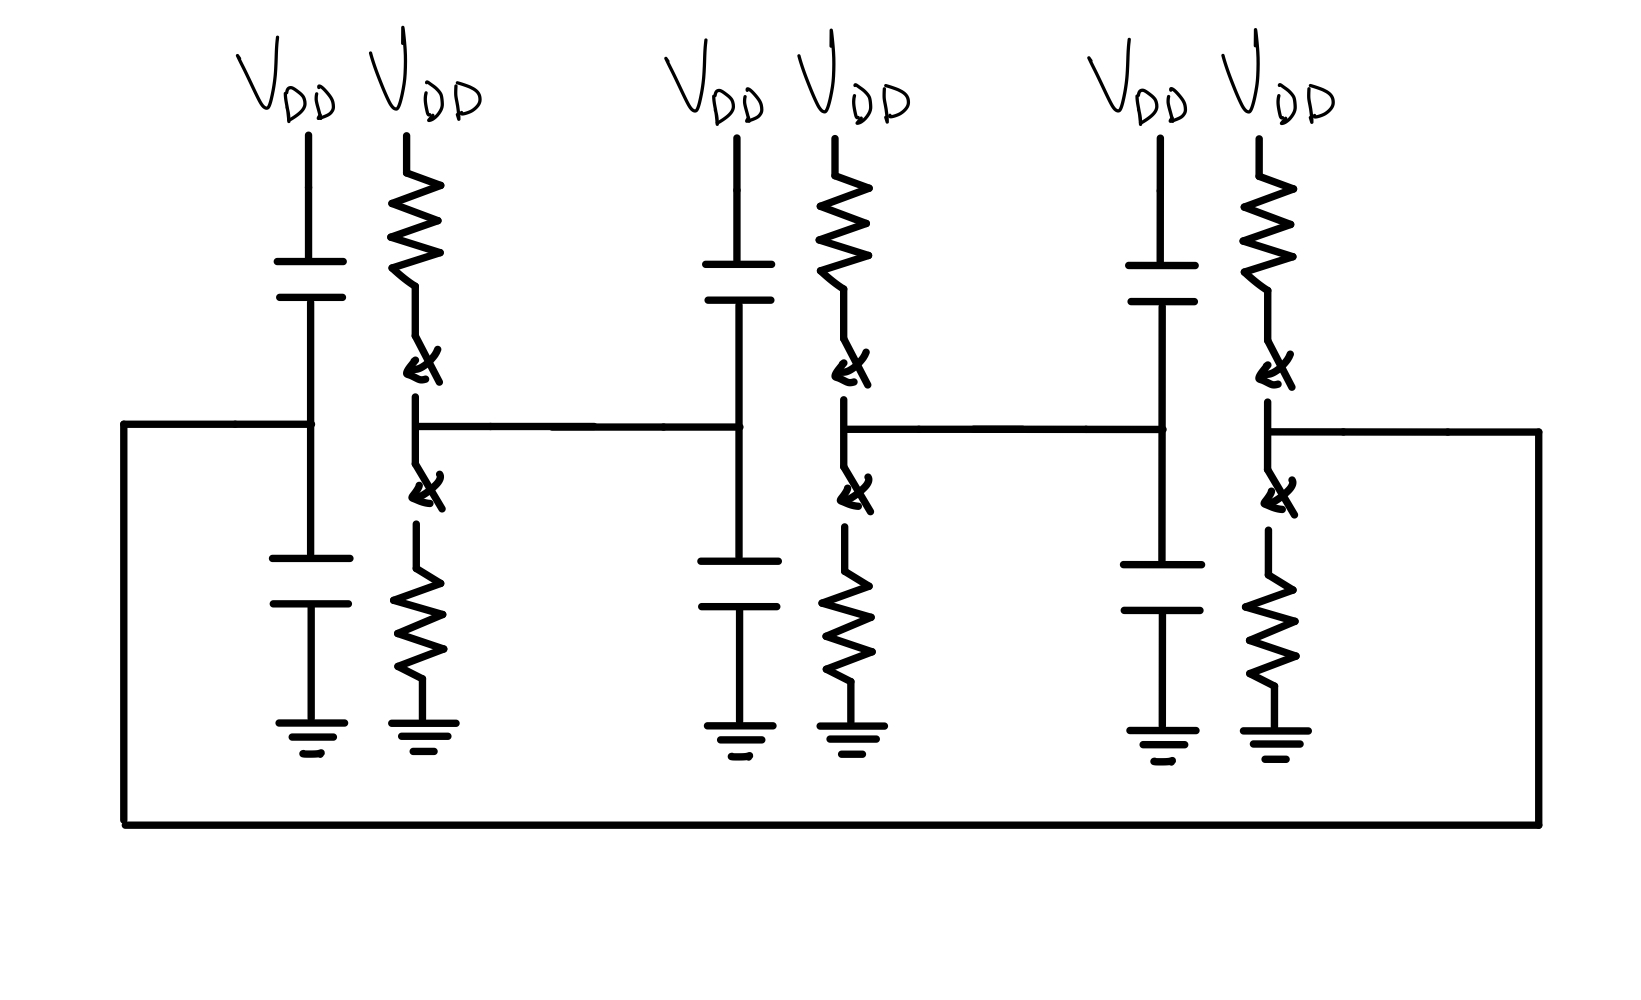
\includegraphics[scale=.15]{01-transistors/detailed-oscillator.jpeg}
    \caption{Detailed ring oscillator with resistor-switch transistor model}
\end{figure}

Let's take a look at specifically the connection between the output of one inverter and the input of the next. When the input voltage to the first inverter is high, the PMOS switch is open and the NMOS switch is closed, making the connection look something like this:

\begin{figure}[H]
    \centering
        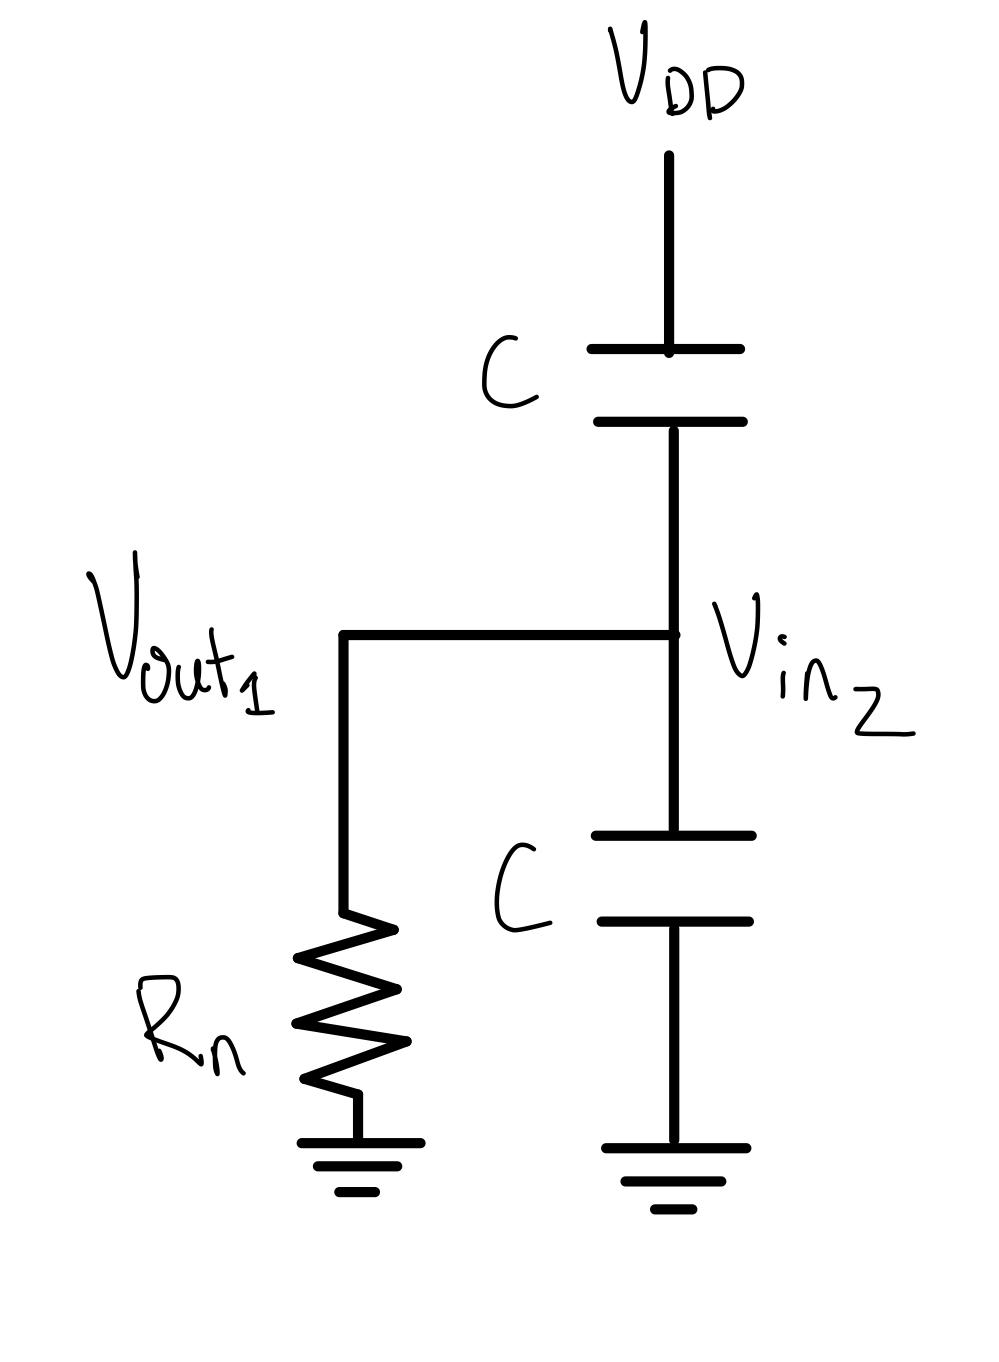
\includegraphics[scale=.1]{01-transistors/inverter-low.jpeg}
    \caption{Inverter low output}
\end{figure}

When the first input voltage is high, the PMOS switch is closed and the NMOS switch is open.

\begin{figure}[H]
    \centering
        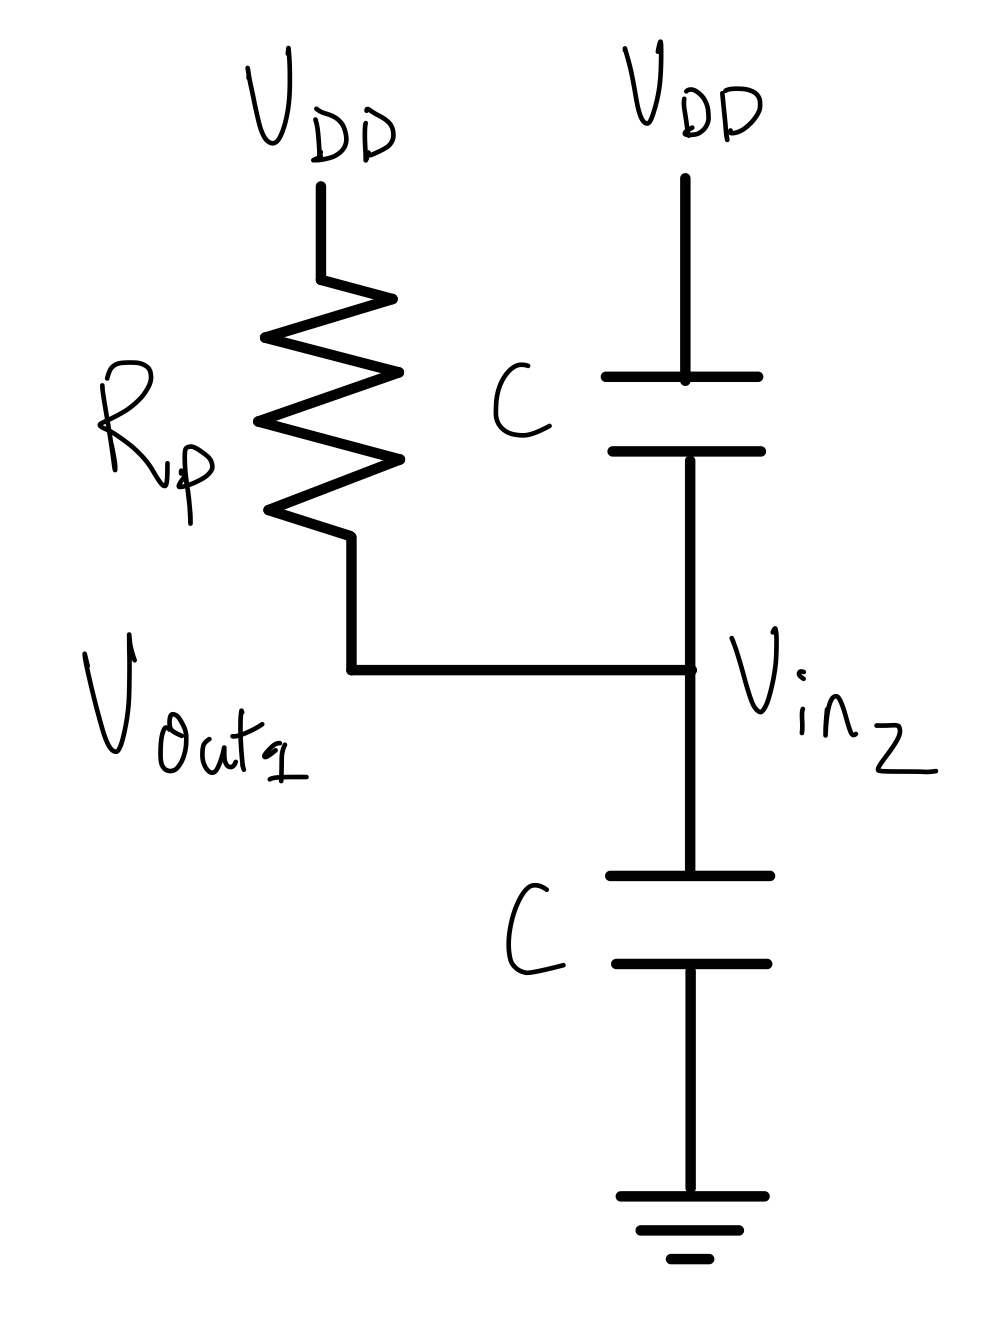
\includegraphics[scale=.1]{01-transistors/inverter-high.jpeg}
    \caption{Inverter high output}
\end{figure}

We can see that the inverters form an RC circuit, charging up the capacitors to the second inverter when the first inverter gives a high output, and discharging the capacitors when the first inverter gives a low output. 

Since this charging and discharging is a gradual process, $V_{in_2}$ does not immediately switch between $V_{DD}$ and $0$, and thus it takes some duration of time after one inverter flips before the next one does.

In the next note, we will explore the behavior of RC circuits like this further using differential equations. 

\end{document}